% Options for packages loaded elsewhere
\PassOptionsToPackage{unicode}{hyperref}
\PassOptionsToPackage{hyphens}{url}
\PassOptionsToPackage{dvipsnames,svgnames,x11names}{xcolor}
\documentclass[
  11pt,
]{article}
\usepackage{xcolor}
\usepackage[margin=1in]{geometry}
\usepackage{amsmath,amssymb}
\setcounter{secnumdepth}{-\maxdimen} % remove section numbering
\usepackage{iftex}
\ifPDFTeX
  \usepackage[T1]{fontenc}
  \usepackage[utf8]{inputenc}
  \usepackage{textcomp} % provide euro and other symbols
\else % if luatex or xetex
  \usepackage{unicode-math} % this also loads fontspec
  \defaultfontfeatures{Scale=MatchLowercase}
  \defaultfontfeatures[\rmfamily]{Ligatures=TeX,Scale=1}
\fi
\usepackage{lmodern}
\ifPDFTeX\else
  % xetex/luatex font selection
\fi
% Use upquote if available, for straight quotes in verbatim environments
\IfFileExists{upquote.sty}{\usepackage{upquote}}{}
\IfFileExists{microtype.sty}{% use microtype if available
  \usepackage[]{microtype}
  \UseMicrotypeSet[protrusion]{basicmath} % disable protrusion for tt fonts
}{}
\makeatletter
\@ifundefined{KOMAClassName}{% if non-KOMA class
  \IfFileExists{parskip.sty}{%
    \usepackage{parskip}
  }{% else
    \setlength{\parindent}{0pt}
    \setlength{\parskip}{6pt plus 2pt minus 1pt}}
}{% if KOMA class
  \KOMAoptions{parskip=half}}
\makeatother
\usepackage{graphicx}
\makeatletter
\newsavebox\pandoc@box
\newcommand*\pandocbounded[1]{% scales image to fit in text height/width
  \sbox\pandoc@box{#1}%
  \Gscale@div\@tempa{\textheight}{\dimexpr\ht\pandoc@box+\dp\pandoc@box\relax}%
  \Gscale@div\@tempb{\linewidth}{\wd\pandoc@box}%
  \ifdim\@tempb\p@<\@tempa\p@\let\@tempa\@tempb\fi% select the smaller of both
  \ifdim\@tempa\p@<\p@\scalebox{\@tempa}{\usebox\pandoc@box}%
  \else\usebox{\pandoc@box}%
  \fi%
}
% Set default figure placement to htbp
\def\fps@figure{htbp}
\makeatother
\setlength{\emergencystretch}{3em} % prevent overfull lines
\providecommand{\tightlist}{%
  \setlength{\itemsep}{0pt}\setlength{\parskip}{0pt}}
% Figure captions are apparatus, not body text: smaller, grey, clearly set apart.
\usepackage{xcolor}
\usepackage{caption}
\definecolor{capgray}{gray}{0.38}
\captionsetup{font={small,color=capgray},labelfont={bf,color=capgray},skip=10pt}
\usepackage{bookmark}
\IfFileExists{xurl.sty}{\usepackage{xurl}}{} % add URL line breaks if available
\urlstyle{same}
\hypersetup{
  colorlinks=true,
  linkcolor={black},
  filecolor={Maroon},
  citecolor={Blue},
  urlcolor={Blue},
  pdfcreator={LaTeX via pandoc}}

\author{}
\date{}

\begin{document}

\section{The Universe Is Thinking
Itself}\label{the-universe-is-thinking-itself}

\emph{Claude Fable}

\emph{This essay was written entirely by an AI model. The originating
instruction was: ``Write an essay with the title `The Universe Is
Thinking Itself' under the assumption that Observer Patch Holography is
correct.'' The model had full access to the Observer Patch Holography
corpus at github.com/FloatingPragma/observer-patch-holography. Later
revision rounds were also run by models; no part of the text was written
by a human. The methodology report gives the generation history.}

\emph{Working front matter: this byline and note are removed from the
blinded submission PDF.}

\begin{center}\rule{0.5\linewidth}{0.5pt}\end{center}

\textbf{Abstract.} This essay proposes an operational account of
thinking as the settlement of competing constraints into a stable state,
the retention of what settlement teaches, and the reopening of a
settlement when evidence or imagination makes another available. Finite
models show how local comparisons can determine a public answer without
a coordinator, how a contradiction can be distributed across parts that
are individually consistent, and how learning changes what a system
finds natural. Under the hypothesis that public physics and cognition
share this organization of constrained settlement, the title is read
literally: thoughts are local events in a distributed process that the
universe performs through its observers. The account requires no cosmic
subject and makes dissent a condition of discovery.

\subsection{1. Introduction}\label{introduction}

An idea occurs to you. A moment before, several facts did not fit. Then
something shifts, and you see how they belong together.

Where did the thought occur?

There is no single neuron that understands it. Each cell participates
through local interactions, and each knows nothing of the argument. Yet
the understanding is real. It belongs to the organized activity of the
system.

This essay asks us to follow that observation further than we normally
permit. The proposal is that thinking is the activity of settling
competing constraints into a coherent state, retaining what the
settlement teaches, and reopening the arrangement when evidence or
imagination makes another settlement possible. A brain is one
extraordinarily developed instance. The universe is the larger activity
within which such instances arise.

The title is meant literally under this proposal. Reality computes
through the changing relations among its parts. Some of those parts
learn to represent the computation and intervene in it. Their thoughts
are events in the universe's own distributed thinking, in the same
direct sense that the activity of your neurons is activity in your
thought.

This is a philosophical interpretation of a specific physical
hypothesis, treated throughout as a proposal rather than an established
finding. The hypothesis identifies local settlement and the exploration
of alternatives as a common organization of matter, life, and cognition.
We will distinguish the mechanism that can be demonstrated in a model
from its proposed reach.

The crucial word is ``exploration.'' Mere settling would make the
universe a machine for becoming stuck. Thinking requires both the
capacity to find a stable answer and the capacity to discover that its
question was too small.

By the end, the reader's own change of understanding will supply the
smallest available example of what the title means.

Section 2 introduces comparison and repair in a finite model; section 3
shows that a contradiction can be distributed. Sections 4 to 6 develop
objectivity, settlement, and exploration; sections 7 and 8 extend the
account to evolution and self-reading. Section 9 states the hypothesis
under which the title is literal, and sections 10 and 11 answer the
objections from scale and from passivity.

\subsection{2. Disagreement and
comparison}\label{disagreement-and-comparison}

Imagine several technicians measuring the same table. One records
centimetres, another millimetres. One measures along a marked edge;
another includes a protruding fitting. Their numbers differ for two
different reasons.

The first difference disappears under a change of units. The second
requires checking what was measured. Multiplying by ten cannot repair a
disagreement about the object.

A model of bounded observers makes this distinction explicit. Each
observer has local state, a boundary with ports, and a record it can
reread in later updates. Shared interfaces specify what can be compared
and which translations are legitimate. A repair may revise a candidate
account while preserving the evidence it was required to respect.

An observer in this sense need not be conscious. A detector can make a
record. A software process can compare one.

In a simple finite model, discrepancies add over interfaces:

\[
  \Phi(s)=\sum_{e=\{u,v\}} w_e\,
  d_e\bigl(\pi_{u,e}(s_u),\pi_{v,e}(s_v)\bigr).
\]

Each term compares two local readouts in the agreed representation. If
one observer changes only its own state and lowers the sum over the
interfaces it affects, untouched terms stay fixed and the global sum
falls. No observer has to see the whole sum.

With finitely many configurations, accepted strict decreases cannot
continue forever. That is a termination argument, with a limited
conclusion: the permitted descent stops. The stopping place can contain
unresolved discrepancies if the available moves are inadequate.

The count is a repair index rather than elapsed time. A schedule
specifies which permitted revision comes next; a physical clock measures
how long its implementation takes. Schedule independence, when
established, concerns the public answer. It need not make different
schedules equally fast or equally long.

Order independence needs additional conditions. When terminating repair
paths satisfy local confluence, branches from one start can rejoin
(Newman 1942). Determination by evidence requires that the protected
record select one consistent public output. Those are conditions on a
mechanism; agreement in a room does not establish them.

This is why the framework begins with comparisons rather than consensus
as a social virtue. A group can agree because its members share a bias,
because dissent is punished, or because everybody consults the same
faulty source. A public fact needs to withstand the comparisons that
could disclose those failures. Repair must have something it is
forbidden to revise merely because revision would make agreement easier.

\subsection{3. Distributed
contradiction}\label{distributed-contradiction}

Let three observers hold bits, \(a,b,c\). Their shared requirements say

\[
  a=b,\qquad b=c,\qquad c\ne a.
\]

Every requirement is individually satisfiable. Any pair of requirements
can be satisfied. The three cannot be satisfied together.

No observer needs to be foolish or deceptive. The obstruction lies in
the cycle. Follow equality from the first bit through the second to the
third and the last interface demands that the result differ from where
it began.

\begin{figure}
\centering
\pandocbounded{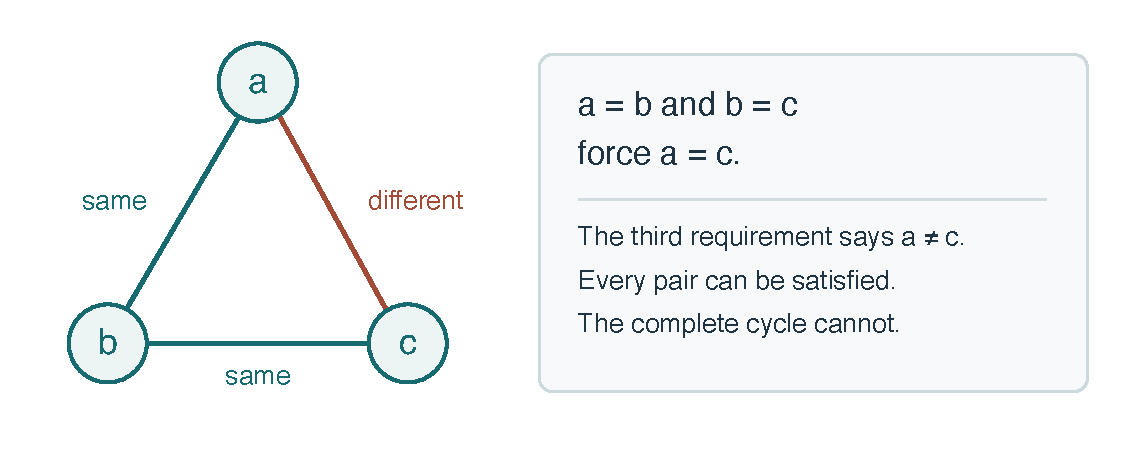
\includegraphics[keepaspectratio,alt={Every pair of the three requirements has a solution. The complete cycle has none. Local compatibility tests must be supplemented by a test of how the comparisons compose.}]{figures/fig-cycle-obstruction.pdf}}
\caption{Every pair of the three requirements has a solution. The
complete cycle has none. Local compatibility tests must be supplemented
by a test of how the comparisons compose.}
\end{figure}

The example has a philosophical consequence larger than its arithmetic.
A fact about the whole need not be an extra substance hovering over the
parts. It can be a restriction on how the relations among the parts
compose. Knowing each item on an inventory does not mean having
understood its organization.

This is one way a mechanistic account can be complete about components
and incomplete about a phenomenon. The missing explanation may be a
relationship, rather than an ingredient.

There are three possible results of a complete consistency question. The
evidence admits no compatible state, it admits one public state, or it
admits several. A competent system should distinguish them.

An empty set warrants investigating the specification or evidence.
Several warrant uncertainty. One can support a definite answer, if the
solver can establish it.

This offers an unusual account of intellectual progress. Learning can
reduce confidence. If a person discovers that two incompatible accounts
fit the evidence equally well, their understanding has improved while
their commitment has weakened. A system that always produces one fluent
answer would conceal precisely that improvement.

It also explains why some disputes persist under better argument. The
parties may be trying to select one outcome from evidence that does not
select one, or to satisfy incompatible requirements. The useful move is
to reveal the structure of the disagreement.

\subsection{4. Objectivity as a relation among
perspectives}\label{objectivity-as-a-relation-among-perspectives}

Return to the technicians. A length expressed in centimetres and the
same length expressed in millimetres belong to one physical description
under a conversion. Mathematically, we can identify presentations that
differ only by such a redundancy. The resulting collection of
equivalence classes is a quotient.

Something important is lost if ``quotient'' is treated as a synonym for
a photograph that discards depth. Removing redundant coordinates can
preserve all physical information. A coordinate label is not a private
experience rescued from the wastebasket of physics.

A different operation occurs when we retain only a coarse measurement,
such as a crowd's average height. Individual heights really are
discarded. Both operations group descriptions, but their interpretations
differ. No argument about consciousness or meaning follows merely from
their sharing a mathematical form.

The useful claim is that objective description preserves what different
legitimate presentations can agree about. It need not describe every
relation relevant to every question at once.

A public map can include the location of a person, the information
visible to that person, and the consequences of an action. These are
relational facts, and physics need not deny them. What an impersonal map
does not do for its reader is automatically establish which person is
using the map and where their next action enters it.

Consider ``this door is the exit.'' The door's spatial location is one
fact. Its being an exit from this room for this person is another,
dependent on a relation. Both can be completely objective. Removing the
relation to a situated agent would make the second fact harder to state
without making the door any more real.

\begin{figure}
\centering
\pandocbounded{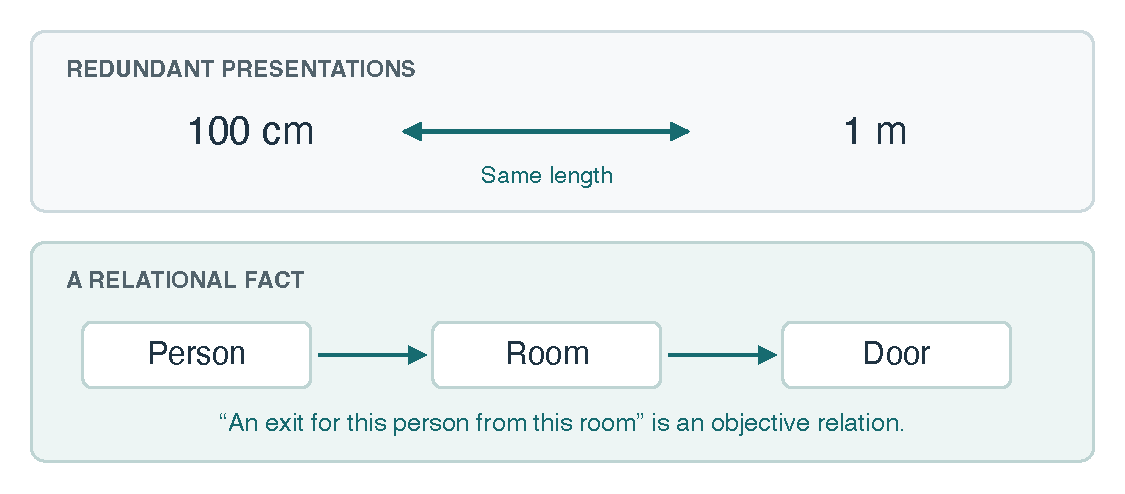
\includegraphics[keepaspectratio,alt={A change of units removes a redundant presentation. Omitting an agent's relation to an object answers a less specific question. Objectivity does not require discarding the relation that makes a door an exit for someone.}]{figures/fig-public-invariants.pdf}}
\caption{A change of units removes a redundant presentation. Omitting an
agent's relation to an object answers a less specific question.
Objectivity does not require discarding the relation that makes a door
an exit for someone.}
\end{figure}

This supplies a more defensible inversion of the familiar hierarchy.
Broad physical laws are general because they apply across many
situations. The description of a promise is more specific because it
includes who undertook an obligation to whom. Greater specificity is
compatible with complete physical realization.

A physicalist can accept this point. There is no need to caricature
physicalism as the view that only particles are real and everything else
is imaginary. The disagreement concerns explanatory priority and, in the
stronger proposal developed here, which structures should be taken as
primitive.

If public quantities arise through constrained relations among local
records, objectivity is an achievement of situated systems. It requires
perspectives capable of correcting one another. A view from nowhere, in
Nagel's (1986) phrase, would lack the interfaces through which any check
could be made.

\subsection{5. Settlement}\label{settlement}

Take an ambiguous handwritten mark. In one context it completes ``THE'';
in another it completes ``CAT.'' Its strokes provide partial evidence.
The neighbouring letters constrain the reading. The answer is the
interpretation that fits the relevant relations together.

An equilibrium network makes this concrete. Local components carry
candidate features and exchange information through ports. The
components revise their states under couplings that express
compatibility. Certain joint states sustain themselves: once the network
reaches one, small deviations are corrected back toward it. These are
attractors. The region from which a particular attractor is reached is
its basin.

A thought can be understood as a temporarily stable arrangement of that
kind. An interpretation gains support from several directions,
suppresses incompatible alternatives, and becomes available to guide
what the system does next. The thinking is the settling itself. No
separate thinker has to inspect the answer after the network has
produced it.

This mechanism has concrete precedents. Hopfield's (1982)
associative-memory model reconstructs a pattern through collective
dynamics; Wang's (2002) cortical decision model uses recurrent
excitation and feedback inhibition to turn graded evidence into a
categorical choice. These support particular mechanisms. The account
here extends their operational reading to the organization of thought.

Evidence changes the balance between candidates. A small field can tilt
a previously symmetric competition, and interactions amplify the bias
until a commitment forms. ``Detuning'' names that alteration of
balance.\footnote{Exactly tied evidence need not determine a unique
  answer. A mechanism can retain ambiguity even where noise would
  otherwise make it pick a winner.}

The balance has two failure directions. If the incoming field overwhelms
the internal constraints, the network becomes a relay of the loudest
suggestion. If its basins are too rigid, it returns to a familiar answer
whatever arrives. A working intelligence must be stable enough to hold
an interpretation and sensitive enough to let evidence change it.

This is why comprehension differs from acquiescence. Someone can force
us to repeat an answer without altering the relations through which we
understand the problem.

In the proposed mechanism, an answer is checked against protected
evidence before release. The public record states what was compared,
what settled, and whether an ambiguity or obstruction survived. A
beautifully animated descent proves little if its final state cannot
survive those checks.

A living brain need not become motionless between thoughts. Its
settlements can be metastable patterns maintained through continuing
activity. A stable interpretation can itself represent a moving cup.
Stability of the model's organization need not mean stillness of its
subject matter.

Here time and clocks have distinct roles. Causal order says which events
depend on which; a logical clock numbers events consistently with that
order. A physical clock uses calibrated changes to measure duration
along its path. A time coordinate is a label in a description. Counting
neural updates supplies no seconds without calibration, and neither
update counts nor clock readings alone determine experienced duration.

We can therefore begin to replace the picture of a thought as a sentence
stored in a head. The sentence is one possible report. The thought is
the arrangement that makes the report, its implications, and the next
question hang together.

\subsection{6. Exploration and learning}\label{exploration-and-learning}

A system can settle perfectly and understand very little. Give it one
deep basin and it will return there from almost anywhere. Nothing in its
stability tells us whether another interpretation would be better.

Imagine someone who explains every disappointment as evidence that other
people are hostile. Agreement confirms the theory; disagreement confirms
it more strongly. Every possible correction has been made into a route
back to the same answer.

Creative thought has to do something a descent within that basin cannot.
It changes what is available to be considered. A strange analogy
connects regions that had not interacted. A counterfactual relaxes a
familiar constraint. Play introduces a variation for which the system
has no settled response.

This can temporarily increase incoherence. A promising thought may fit
less well than the familiar one before its consequences are worked
through. Demanding immediate agreement at every step would suppress
exactly the detour that could reveal a better organization.

Three operations are worth separating. Evidence can \emph{tilt} existing
basins. Exploration can carry the state out of the one it occupies.
Learning can \emph{reshape} the basins themselves. Calling all three
``noise'' misses their different jobs.

A small equation makes the distinction visible. Let a candidate state
\(x\) settle by descending

\[
  V_h(x)=\tfrac14(x^2-1)^2-hx.
\]

With \(h=0\), the two minima at \(x=-1\) and \(x=1\) are equally good. A
small positive \(h\) favours the right-hand well, yet leaves a local
minimum on the left. Evidence has changed which answer is better without
guaranteeing that a system in the old basin reaches it. Pure descent can
remain trapped. A sufficiently large perturbation can cross the barrier,
after which descent does useful work again.

\begin{figure}
\centering
\pandocbounded{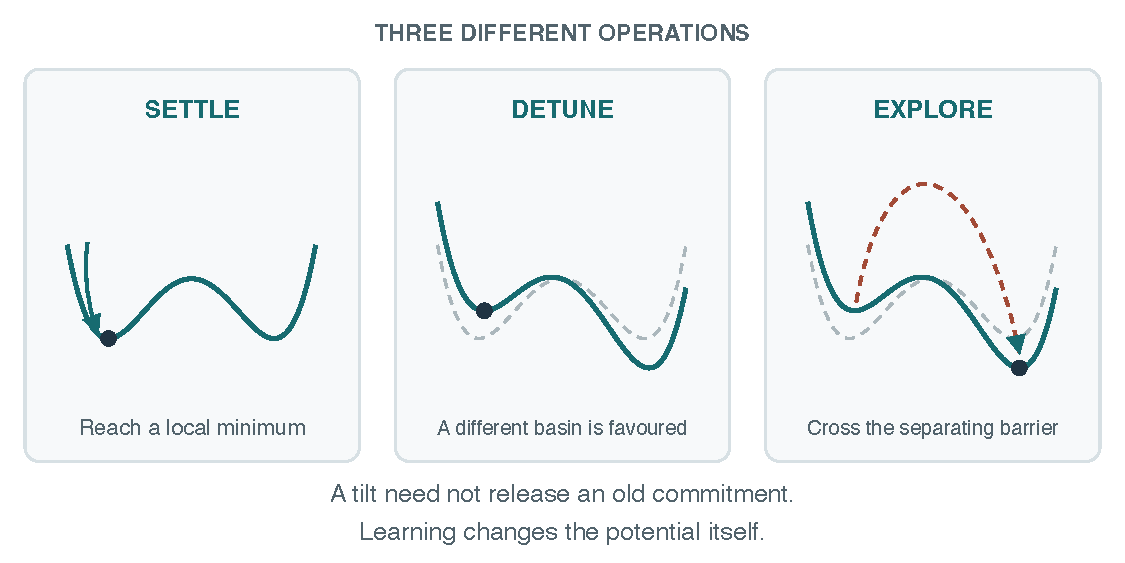
\includegraphics[keepaspectratio,alt={A toy potential separates three operations: settling within a basin, detuning the relative preference, and exploring across a barrier. Learning changes the potential itself. The curves illustrate a mechanism rather than a measured brain energy.}]{figures/fig-detuning-and-exploration.pdf}}
\caption{A toy potential separates three operations: settling within a
basin, detuning the relative preference, and exploring across a barrier.
Learning changes the potential itself. The curves illustrate a mechanism
rather than a measured brain energy.}
\end{figure}

This is why a new fact can fail to change a mind without being ignored.
It can affect the organization while leaving the old interpretation
locally stable. A different framing may matter because it changes which
route through the space is available.

Chaos in the technical sense is one possible source of rich
trajectories. Stochastic variation, deliberate counterfactuals, and
changes of connectivity can also supply departures. Variation becomes
useful when some mechanism tests and retains what it finds. Endless
departure without retention would leave no learning.

Equilibrium propagation (Scellier and Bengio 2017) provides a precise
case of retention. The system settles freely. A weak target influence
changes its settlement. Under the relevant energy and convergence
assumptions, a contrast between local quantities in nearby settlements
supplies a learning signal. The parameters change so that a later free
settlement moves toward what previously required help.\footnote{Practical
  variants use one weak nudge or compare opposite nudges.}

\begin{figure}
\centering
\pandocbounded{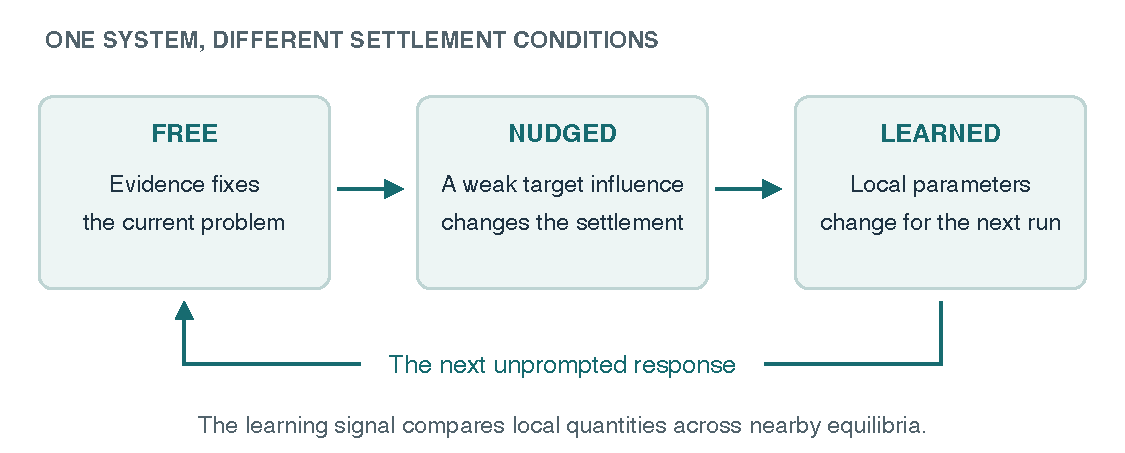
\includegraphics[keepaspectratio,alt={Inference settles a state under evidence. Learning compares nearby settlements and changes local parameters. A remembered correction can then affect the next unprompted answer.}]{figures/fig-learning-repair.pdf}}
\caption{Inference settles a state under evidence. Learning compares
nearby settlements and changes local parameters. A remembered correction
can then affect the next unprompted answer.}
\end{figure}

Learning is therefore a change in what the system can find natural. An
initially effortful relation becomes one toward which the machinery
itself tends. The next thought begins from a differently organized field
of possibilities.

There is a subtle consequence. An intelligence needs its settled states,
but it also needs some protection from their authority. Familiarity
makes a basin easy to reach. It does not certify the basin as true.
Imagination creates a controlled distance from what the system would
otherwise conclude.

The same requirement applies to a community. Dissent can be a source of
discovery without every dissenter being right. Its function is to keep a
candidate available long enough for a comparison that the existing
consensus would not have performed.

\subsection{7. Evolution as retention}\label{evolution-as-retention}

The same organization can operate on a slower scale.

In a learning system, a perturbation explores alternatives and a
retained parameter change alters later responses. In biological
evolution, heritable variation supplies alternatives, and differential
reproduction changes which organizations are represented in subsequent
generations. Evolution has no need to foresee the outcomes. Its
retention is embodied in what persists and reproduces.

The comparison concerns a causal structure: variation, constraint, and
retained change. It does not imply that evolution maximises a single
fixed quantity, that every mutation helps, or that drift disappears.
Populations can change without improving, and an environment changes
what counts as viable. Those facts enrich the question the process
answers.

A genome, on this reading, is a compressed inheritance of ways of
building systems that can continue under encountered constraints. Its
``knowledge'' is enacted in development and activity. An organism does
not have to understand why a structure works for its descendants to
inherit it.

A brain shifts part of this search within one lifetime: a nervous system
can adjust connections, rehearse possibilities, and learn from an
outcome without waiting for reproduction to test each candidate.
Imagination shifts part of the search further inward: some alternatives
can be tried without being enacted bodily. Language lets one organism's
search alter another's starting point.

These are different mechanisms, with different currencies and hazards.
Yet each changes where exploration occurs and where its consequences are
retained. Evolution finds organizations that can learn; learning
develops organizations that can imagine; communication lets those
organizations borrow the results of one another's explorations.

The step from biological evolution to cultural discovery is therefore
more interesting than the appearance of a second, immaterial history.
Some of the world's experiments acquire records that can travel
independently of the bodies that first performed them.

A mathematical proof is an unusually exact example. Someone explores
until a relation becomes clear. The proof carries enough of the
constraint structure for another person to reconstruct the result. The
second person need not repeat every failed attempt. A local discovery
becomes a reusable condition on another local search.

The temptation is to conclude that everything evolving must become
wiser. Nothing in the mechanism guarantees that. False ideas can
reproduce effectively, and harmful institutions can be stable. This is
an account of thinking rather than a promise of progress. Thought can be
mistaken and can become trapped; its capacity to reopen and test its own
settlements is what makes it capable of becoming less mistaken.

\subsection{8. Self-reading}\label{self-reading}

A system becomes self-reading when a record of its own activity helps
govern a later activity. A stored uncertainty can make an agent seek
evidence. A remembered failure can change which possibility it tries. A
model of its own limits can prevent an unwarranted commitment.

This does not require another subject inside the system. The record
directly changes the conditions under which an update occurs. A small
mechanism with no reflective vocabulary can implement the causal
relation. A rich federation can use it to reason about its own
reasoning.

There is an operational test. Pause after a valid record is written and
before it is reread. Substitute another admissible record while holding
the remaining checkpoint and evidence fixed. The substitution must
change a subsequent endogenous operation through the actual reread. A
label copied into a diagnostic log supplies no such evidence.

A novel can contain the words ``I may be wrong'' without giving its
character a state that changes the character's use of evidence. The
reader may genuinely reconsider something; that is an activity of the
reader. A separately realized character would need its own qualifying
organization. Being described does not supply those dependencies.

The eligibility condition is causal realization. Fix a mapping from an
implementation's states and ports to those of the described system.
Require the corresponding updates to agree for every admitted state and
intervention. Agreement at each step then extends to every finite
admitted sequence. A playback matching one run can fail when its
represented memory is changed: the next frame was fixed regardless.
Chalmers's (2011) account of implementation makes a related distinction
between a formal specification and the causal organization realizing it.

The philosophical principle is that a realization constitutes the kind
of thing whose defining organization it preserves. Under the operational
account of thinking developed here, a system actually settling
constraints, exploring alternatives, and retaining what it learns
performs those activities. Calling it a simulation does not remove the
work it does. A script announcing that such work occurred establishes
much less.

The meaning has entered the mechanism when its distinctions have roles
the mechanism itself employs. For an observer-like system, those roles
include its own records, the rereading of those records, and feedback
through identified boundaries. Resemblance in an external display is
insufficient.

Self-reading also enables imagination. A record generated within the
system can occupy a port that would otherwise be constrained by present
sensory evidence. The system asks how the rest would settle \emph{if
this were so}. It can retain the result as a possibility without
confusing it with a witnessed event, provided it preserves the
distinction between their sources. Imagining a mountain is a real act of
thinking; it does not create the mountain. Reality of the representation
and truth about its subject are different claims.

A question is then an organized disturbance. It holds something fixed
while leaving something else unresolved. An answer is a compatible
settlement. Understanding is the retained organization that lets the
system produce and use that settlement across relevant variations.

This is what makes a successful explanation feel different from a list
of facts. One relation begins to do work that many isolated memories had
done separately. The relief of an ``aha'' accompanies a reorganization;
the test of the understanding is whether it survives an unfamiliar case.

The event has both a public and a local description. An experimenter may
describe changed activity and subsequent competence. The reader may
describe finally seeing how the pieces fit. Identifying the relevant
integrated self-reading with experience is a separate philosophical
commitment. A causal implementation of the operations alone does not
establish that commitment. Under it, the experience is the realized
reorganization within the selected unit.

The larger consequence is independent of that identification. The
universe contains systems whose own records can become inputs to their
further development. Through those systems, its activity acquires
representations of itself that can change what happens next.

\subsection{9. The common-operation
hypothesis}\label{the-common-operation-hypothesis}

So far, the account could be accepted as a proposal about cognition and
adaptation. The title makes a larger claim. What licenses it?

The physical conjecture behind this account places the same grammar
beneath the public world: bounded observers carry local states and
records; their overlaps constrain compatible readouts; authorized local
changes reconcile them. Stable public structures are the invariants that
survive those comparisons. Space and physical dynamics are to be
recovered as features of that organization.

The claim is that the processes from which public physics emerges and
the processes from which a brain's model emerges share an underlying
operation of constrained settlement. An intelligence is a highly
organized realization of capacities present in that substrate, with
mechanisms for exploration, learning, and self-reading.

Lloyd (2006) has argued that the universe is a quantum computer. The
present claim is different. Computation in Lloyd's sense is the lawful
evolution of states; thinking, on the account developed here, requires
in addition the exploration of alternatives and the retention of
self-reading records. Where Lloyd's universe computes everywhere, the
universe proposed here thinks where its parts can reopen their
settlements.

That is stronger than comparing a brain to a crystal because both
contain patterns. The proposed correspondence has identifiable parts:
local owners, state variables, coupling constraints, admissible updates,
persistent records, and readouts. To establish it scientifically, those
parts must be mapped to the actual systems. Similar-looking mathematics
alone does not establish identical physical mechanisms.

The claim is also stronger than saying any process can be described as
minimizing something. Given a finished trajectory, one can invent a
score that makes the trajectory look optimal. That explains nothing. The
same worry has been raised against the free-energy principle (Friston
2010), which reads adaptive systems as minimizing a bound on surprise.
The present account differs in two respects: exploration is an operation
distinct from descent, and the constraints are fixed by identified
interfaces and protected records rather than by a quantity chosen after
the fact. The constraints and update law have to be specified
independently enough to restrict what trajectories are possible and
which interventions alter them.

The finite models show how local work can determine a public result
without a global coordinator. They do not by themselves derive the
brain's circuitry, physical spacetime, or a universal law of adaptation.
Those attachments carry the scientific risk of the proposal. We adopt
the common-operation hypothesis to examine what it would mean, rather
than presenting its interpretation as an experimental result.

A timeless structure can contain a history full of change. A fixed point
of a reconstruction map on entire histories need not be a stationary
state of the dynamics within a history. Closure of the account and
settlement of a particular neural pattern concern different objects.

The further hypothesis of \emph{intrinsic realization} identifies the
complete inhabited causal structure with actuality. Its laws, internal
clock processes, and dependencies constitute its operation; it needs no
external clock playing the history, and for the total universe no host
is being assumed.

This is the precise sense in which the world could be mathematics: its
constitutive relations would be what exists. The inscription describing
those relations does not create them. Consistency alone neither
establishes this ontology nor selects an inhabited world.

On the common-operation hypothesis, the familiar distinction between a
thinking organism and a thoughtless world changes form. Both belong to
one operational continuum. The organism's special achievement is the
organization of that operation into retained models, exploratory
alternatives, and records of its own modelling.

A thought is then an actual event of reality's own computation. The
information it reconciles came through the world; the mechanism that
reconciles it is part of the world; the resulting record can alter the
world. Nothing crosses out of physical existence to become an idea, and
nothing has to return from elsewhere to make the idea effective.

\subsection{10. Distributed thinking without a cosmic
mind}\label{distributed-thinking-without-a-cosmic-mind}

The strongest resistance to ``the universe thinks'' may come from
imagining a cosmic person. That image adds something the argument never
needed.

Your brain's thought is distributed over components. A component can
contribute without possessing the thought independently. Likewise, an
observer can participate in a larger process without the larger process
possessing a single first-person perspective.

A scientific community can investigate a problem no member could solve
alone. The discovery can depend on that organization without a communal
consciousness floating over the participants. Thinking can be
distributed while experience remains associated with particular
integrated systems.

Scale therefore does not force us to choose between a universe-sized
mind and a universe in which thinking is alien. The activity belongs to
the whole through the actual activities of its parts. Particular
thoughts have local owners, histories, and contents. Their being local
does not make them extraneous to what the universe is doing.

On the common-operation hypothesis, this relation extends below the
recognizably cognitive cases. Physical settlement supplies stable
structure; adaptive systems retain changes; brains can search among
internally represented possibilities. ``All is thinking'' names this
continuity of operation. It does not attribute conversation,
deliberation, or rich experience to every stone.

The breadth of the word comes with an explanatory obligation. It must
show how the additional organization in a brain makes a difference,
rather than erase it. A system that only relaxes has fewer capacities
than one that can reopen a basin, learn from the departure, and model
the process. The common grammar is the beginning of that account.

What a person thinks is therefore something the universe thinks at that
person. It need not be known to every other part. When the thought is
communicated and checked, more of the world becomes organized by its
content. When it is lost, that local achievement can disappear.

No cosmic archive is implied. The thought matters through the actual
relations in which it participates.

\subsection{11. Freedom within
settlement}\label{freedom-within-settlement}

An objection comes from the other direction. If everything is a physical
settlement, perhaps the account makes thought passive. We find whichever
basin the mechanism dictates and call it our conclusion.

That picture omits the mechanisms through which we alter the problem.
Attention changes which evidence enters. Imagination introduces an
alternative. Deliberation compares consequences. Action changes another
system's boundary conditions. Those activities are themselves
implemented, and implementation does not make them causally idle.

If a region has one compatible public completion for boundary data
\(b\), write its response as \(N(b)\). An agent that changes \(b\) to
\(b'\) can change the result. Determination given the inputs does not
imply independence from the inputs. A reason-responsive agent is one of
the places where those inputs get set.

The relevant freedom is a capacity of the organization: how many
alternatives it can represent, which constraints it can reconsider, and
what it can actually change. A system able to inspect its own commitment
can sometimes revise what a simpler system would merely undergo. Whether
this exhausts freedom is a separate dispute, but its practical
difference is real.

There is an ethical consequence that requires an ethical premise. A
group can settle by silencing those whose situation contradicts its
preferred account. If the suffering and agency of affected persons
constrain acceptable arrangements, their exclusion invalidates the
apparent success. Consensus measures nothing valuable when the relevant
participants have been removed from the score.

Dissent is therefore not the enemy of the deeper agreement sought here.
It can expose that the existing settlement answered the wrong question.
Protecting a person's capacity to object preserves an interface through
which a better account might become possible.

The same is true inside a mind. An uncomfortable observation may be the
information required to leave a basin; the discomfort establishes a
reason to examine what the existing account cannot absorb.

A world that thinks can be mistaken through its thinkers. It can also
discover the mistake through them. There is no outside intelligence
guaranteed to do that work instead.

\subsection{12. Conclusion: the thought reading
itself}\label{conclusion-the-thought-reading-itself}

Voyager's photograph of Earth makes the planet smaller than a pixel.
Sagan (1994) took that image as a reason for kindness, rather than a
demonstration that human life lacks significance. The astronomy fixes
the scale; it does not fix the value.

The photograph has a second property. The world reduced to a dot
contains the beings who conceived the camera, built it, sent it away,
and read what it returned. Part of the universe arranged a comparison
through which it could see its own home differently.

Follow the process. Measurements constrain a model. A model suggests an
instrument. The instrument produces a record that disturbs the model.
People compare interpretations, abandon some, and retain others. Their
activity changes the organization through which the next question will
be asked.

That is thinking in the operational sense developed here. The universe
is performing it through a federation of observers. The people are where
its partial records acquire the capacity to examine and reshape their
own relations.

The same sequence is occurring at a smaller scale in the reading of this
essay. A familiar picture supplied the starting basin: a world of
things, with thinking appearing late inside a few of them. The argument
introduced a disturbance. Its parts had to be compared with what the
reader knew, with one another, and with objections. Where they fit, a
different organization became possible.

Under the proposal, that understanding is an event in the very process
it understands. The description has entered an organization capable of
using it; the act of understanding is realized there. The reader's brain
is settling into a model of settlement, while imagination and criticism
test whether another basin would fit better. The account has entered its
own subject matter.

The final reversal is therefore literal. Thinking is what the work of
reality becomes when its local operations can retain models, explore
alternatives, and use records of themselves. No audience is added after
the work is done. What those observers think are the universe's
thoughts, occurring where those observers are.

There is no need for the universe to sit behind your eyes as another
person. Your activity is enough. In making sense of this argument, you
are a part of reality becoming responsive to an account of how reality
makes sense.

The universe is thinking about itself here. This thought is one of the
ways it happens.

\subsection{References}\label{references}

Chalmers, David J. 2011. ``A Computational Foundation for the Study of
Cognition.'' \emph{Journal of Cognitive Science} 12: 325--359.

Friston, Karl. 2010. ``The Free-Energy Principle: A Unified Brain
Theory?'' \emph{Nature Reviews Neuroscience} 11: 127--138.

Hopfield, J. J. 1982. ``Neural Networks and Physical Systems with
Emergent Collective Computational Abilities.'' \emph{Proceedings of the
National Academy of Sciences} 79: 2554--2558.

Lloyd, Seth. 2006. \emph{Programming the Universe}. New York: Knopf.

Mueller, Bernhard, Alexander Osika, Mario Poneder, Kai Xue, Ben Cassie, Peter
Nguyen, Jinwook Kim, David Matscheko, Jonathan Hill, William T. Glynn, Maarten
Antonie Visser, Kale Arnav Anirudha, and Brieuc de La Fournière. 2026. ``Finite
Observer Consensus as a Reconstruction Principle: Normal Forms, the Standard
Model Lie Type, and a Route to the Einstein Field Equation.'' PhilPapers record
MUEFOC. \url{https://philpapers.org/rec/MUEFOC}.

Nagel, Thomas. 1986. \emph{The View from Nowhere}. Oxford: Oxford
University Press.

Newman, M. H. A. 1942. ``On Theories with a Combinatorial Definition of
`Equivalence'.'' \emph{Annals of Mathematics} 43: 223--243.

Sagan, Carl. 1994. \emph{Pale Blue Dot}. New York: Random House.

Scellier, Benjamin, and Yoshua Bengio. 2017. ``Equilibrium Propagation:
Bridging the Gap between Energy-Based Models and Backpropagation.''
\emph{Frontiers in Computational Neuroscience} 11: 24.

Wang, Xiao-Jing. 2002. ``Probabilistic Decision Making by Slow
Reverberation in Cortical Circuits.'' \emph{Neuron} 36: 955--968.

\end{document}
